\documentclass[11pt,a4paper]{article}
\usepackage[margin=24mm]{geometry}
\usepackage[T1]{fontenc}
\usepackage{lmodern}
\usepackage{amsmath,amssymb,booktabs,array,microtype}
\usepackage{tikz}
\usetikzlibrary{arrows.meta,positioning,calc,fit}
\usepackage{hyperref}
\hypersetup{colorlinks=true,urlcolor=black,linkcolor=black}
\usepackage{caption}
\captionsetup{font=small}
\title{\bfseries Supplementary Information S1\\[4pt]\large Computational Pipeline, Numerical Reproducibility and Parameter Selection}
\author{\parbox{0.92\textwidth}{\centering\small Companion to: \emph{Can Non-Gaussian Residuals Enable Remote Detection of a Laser Beam Perturbation along Its Propagation Path?}}}
\date{}
\begin{document}
\maketitle
\noindent\textbf{Scope.} This document describes the numerical architecture, parameter-selection history, stochastic ensemble design, statistical workflow, and reproducibility considerations underlying the manuscript. The investigation is a numerical proof of principle; no laboratory detection performance is claimed.

\section{Computational framework}
The incident optical field is represented by a coherent Gaussian transverse amplitude,
\begin{equation}
 E_0(x,y)=E_{00}\exp\!\left[-\frac{x^2+y^2}{w_0^2}\right],
 \label{eq:input}
\end{equation}
where $w_0$ denotes the beam-radius parameter. A localized, thermally inspired perturbation is modeled as a spatially correlated phase screen rather than by solving coupled thermal-fluid and optical equations. For each nonzero perturbation strength $\phi_0$, independent unit-variance Gaussian noise $\xi(x,y)$ is spatially smoothed, mean-centered and standardized to give $\eta(x,y)$. The implemented phase screen is
\begin{equation}
 \phi(x,y)=\phi_0\,\exp\!\left[-\frac{x^2+y^2}{p_z^2}\right]
 \frac{\eta(x,y)}{\operatorname{std}[\eta]},\qquad
 \eta=G_{\sigma_{\rm pix}}*\xi-\left\langle G_{\sigma_{\rm pix}}*\xi\right\rangle,
 \label{eq:screen}
\end{equation}
with Gaussian-filter smoothing scale $\sigma_{\rm pix}$ in pixels. In the implementation the filter uses reflecting boundary conditions. The phase-modulated input field is $E_{\rm on}(x,y;0)=E_0(x,y)\exp[i\phi(x,y)]$; the reference is $E_{\rm off}(x,y;0)=E_0(x,y)$.

Propagation through distance $z$ is computed using the FFT-based Fresnel transfer function
\begin{equation}
 E(x,y;z)=\mathcal{F}^{-1}\!\left\{\mathcal{F}[E(x,y;0)]\,
 \exp\left[-i\pi\lambda z(f_x^2+f_y^2)\right]\right\},
 \label{eq:fresnel}
\end{equation}
where $f_x,f_y$ are transverse spatial frequencies. The recorded numerical observables are the propagated intensities $I_{\rm on/off}=|E_{\rm on/off}|^2$. Global phase factors, which cancel from intensity, are omitted in the transfer function. This model isolates propagation-induced intensity signatures of a stochastic phase perturbation; it is not a full model of an atmospheric or laboratory thermal plume.

\section{Physical and numerical parameters}
\begin{table}[htbp]
\centering\small
\caption{Parameters of the consolidated numerical configuration. The phase-filter width is specified in pixels in the executable notebook; its millimetre equivalent is derived from the sampling interval.}
\label{tab:parameters}
\begin{tabular}{@{}p{0.35\linewidth}p{0.32\linewidth}p{0.24\linewidth}@{}}
\toprule
Quantity & Symbol / notebook variable & Value\\ \midrule
Grid size & $N$ & $1024\times1024$\\
Transverse domain width & $L_x$ & $80\,\mathrm{mm}$\\
Gaussian beam radius & $w_0$ & $10\,\mathrm{mm}$\\
Wavelength & $\lambda$ & $532\,\mathrm{nm}$\\
Propagation distance & $z$ & $0.60\,\mathrm{m}$\\
Phase-filter Gaussian width & \texttt{FILTER\_SIGMA\_PIXELS} & $18$ pixels ($\simeq1.41\,\mathrm{mm}$)\\
Perturbation envelope scale & $p_z$ & $107\,\mathrm{mm}$\\
Perturbation strengths & $\phi_0$ & $0,0.05,0.10,0.20,0.30,0.50\,\mathrm{rad}$\\
Independent realizations & \texttt{N\_REALIZATIONS} & $100$ per nonzero $\phi_0$\\
Random master seed & \texttt{MASTER\_SEED} & $2026$\\
Profile extraction & \texttt{STRIP\_HALF\_WIDTH} & $4$ pixels (9 rows total)\\
\bottomrule
\end{tabular}
\end{table}
The grid spacing is $\Delta x=L_x/(N-1)\simeq0.0782\,\mathrm{mm}$. Accordingly, $18\Delta x\simeq1.41\,\mathrm{mm}$. This is the \emph{Gaussian-filter standard deviation} used to generate the phase texture, not an independently measured experimental turbulence correlation length. Similarly, $p_z=107\,\mathrm{mm}$ characterizes the broad Gaussian envelope in Eq.~\eqref{eq:screen}; it does not denote the longitudinal propagation distance.

\section{Development of the numerical experiments and parameter selection}
The computational study evolved through five exploratory configurations. In experiments E1 and E2, the physical and numerical input parameters were varied to identify a configuration producing interpretable propagation patterns and residual signatures. The values in Table~\ref{tab:parameters} were retained following this exploratory stage. Experiments E3 and E4 introduced Monte Carlo sampling to assess realization-to-realization variability, rather than relying exclusively on individual phase-screen examples. Experiment E5 consolidated the selected input configuration and the ensemble-based statistical workflow used for the manuscript.

This history describes the sequence of model development, not a formal optimization algorithm. The earlier exploratory configurations have not been supplied as an independently archived parameter sweep; consequently, no quantitative convergence, optimality, or sensitivity claim is made for E1--E4. In particular, the final parameter values should not be interpreted as uniquely optimal or experimentally calibrated. Their role is to specify a reproducible, physically motivated proof-of-principle scenario suitable for informing future experimental design.

\section{Monte Carlo design and computational pipeline}
For each nonzero phase amplitude, the model generates $100$ independent correlated phase screens and repeats propagation and downstream statistical analysis. The zero-perturbation OFF reference is deterministic in the implemented model and is computed once, rather than treated as a separate stochastic ensemble. A fixed master seed controls reproducible pseudorandom sampling.

\begin{figure}[htbp]
\centering
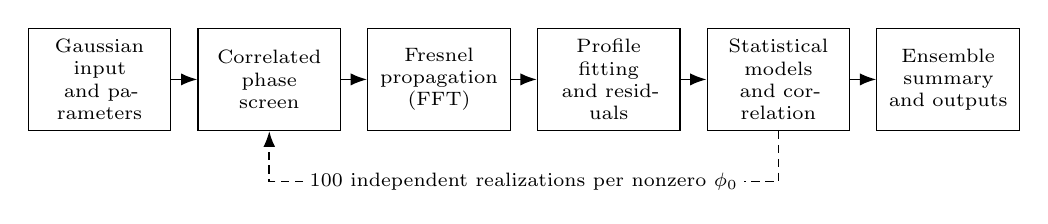
\begin{tikzpicture}[>=Latex, node distance=3.3mm,
 block/.style={draw=black,rounded corners=0pt,align=center,minimum height=13mm,text width=0.132\linewidth,inner sep=3pt,font=\scriptsize},
 arr/.style={-Latex,line width=.65pt}]
\node[block] (a) {Gaussian input\\and parameters};
\node[block,right=of a] (b) {Correlated phase\\screen};
\node[block,right=of b] (c) {Fresnel propagation\\(FFT)};
\node[block,right=of c] (d) {Profile fitting\\and residuals};
\node[block,right=of d] (e) {Statistical models\\and correlation};
\node[block,right=of e] (f) {Ensemble summary\\and outputs};
\foreach \u/\v in {a/b,b/c,c/d,d/e,e/f} \draw[arr] (\u.east)--(\v.west);
\draw[densely dashed, -Latex, line width=.6pt] (e.south) -- ++(0,-.64) -| (b.south);
\node[font=\scriptsize,fill=white,inner sep=2pt] at ($(b.south)!0.5!(e.south)+(0,-.64)$) {100 independent realizations per nonzero $\phi_0$};
\end{tikzpicture}
\caption{Computational pipeline for the numerical study. Each stochastic phase-screen realization undergoes FFT-based Fresnel propagation, profile extraction, residual analysis and statistical characterization. The ensemble is then aggregated into summary statistics, machine-readable tables and manuscript figures. The deterministic unperturbed reference is evaluated separately.}
\label{fig:pipeline}
\end{figure}

As shown in Fig.~\ref{fig:pipeline}, a narrow transverse profile is extracted by averaging nine central image rows. A Gaussian profile is fitted to characterize the reference beam shape, and the departures from that fitted profile are used to construct the residual-based observables. The ensemble treatment preserves the distinction between independent realizations and correlated spatial samples within a single realization.

\section{Statistical characterization}
The analysis computes distributional moments, including skewness and excess kurtosis, of the relevant standardized residuals. Candidate probability models include the normal, Student-$t$ and generalized-normal families. Their parameters are fitted to each realization, rather than treating all spatial residual samples from all realizations as a single independent pooled dataset. The Akaike information criterion is calculated as
\begin{equation}
 \mathrm{AIC}=2k-2\log\widehat{L},
 \label{eq:aic}
\end{equation}
where $k$ is the number of fitted model parameters and $\widehat{L}$ the maximized likelihood. Smaller AIC indicates a preferable fit within the compared candidate set under the AIC criterion; it is not proof of a unique physical residual-generation mechanism. The notebook also calculates BIC for the candidate fits.

Spatial autocorrelation of the transverse residual structure provides complementary information about characteristic spatial scales. The implementation uses an $e^{-1}$ autocorrelation threshold for the reported correlation-length convention. Such a length is a descriptor of the simulated residual pattern, and should not be conflated with the phase-filter smoothing width specified in Table~\ref{tab:parameters}.

\section{Computational implementation and reproducibility}
The reference implementation is provided as a Python notebook intended for Google Colab. The main computational burden comes from repeated two-dimensional field operations, including Gaussian filtering of $1024\times1024$ random arrays and FFT-based propagation, together with iterative probability-distribution fits for the ensemble of realizations. These operations are plausible contributors to runtime; their individual shares have not yet been established by a profiler.

The observed end-to-end runtime in Google Colab is approximately \textbf{11 minutes}, with the main simulation and statistical analysis accounting for nearly all of that duration. Generation of the manuscript figures from the computed results is comparatively fast. Actual runtime depends on Colab's allocated resources and installed numerical-library versions; the 11-minute value is an observation, not a performance guarantee or benchmark. The notebook should be executed sequentially from a clean runtime.

The reproducibility package is designed to contain the executable notebook, dependency information, machine-readable CSV results, manuscript figures and a README describing execution. At the time of preparing this document, repository and archival identifiers should be added only after public release; no unassigned GitHub URL or Zenodo DOI is asserted here.

\section{Parameter sensitivity, limitations and experimental outlook}
The selected configuration illustrates how correlated phase perturbations can generate measurable changes in propagated beam structure and in residual-based statistics. It does not establish performance over the full range of beam radii, propagation distances, grid sizes, perturbation envelopes, phase amplitudes or correlation scales. A formal one-at-a-time or global sensitivity analysis remains a useful extension, especially for assessing detection thresholds and numerical convergence.

The phase screen is phenomenological and thermally inspired; the model does not simulate temperature transport, refractive-index fluctuations from fluid dynamics, detector noise, camera sampling, mechanical alignment errors, or a complete optical apparatus. Accordingly, simulation-derived statistical separability must be distinguished from experimental detection sensitivity. A future laboratory campaign should independently vary controllable optical and perturbation parameters, characterize instrument noise, and test whether the proposed residual statistics discriminate perturbed and unperturbed conditions under realistic uncertainty.

\section*{Reproducibility note}
The computational implementation and generated datasets constitute the definitive specification of the reported numerical procedure. If a descriptive equation or summary in this supplement is interpreted differently from the executable implementation, the latter should be consulted and any discrepancy resolved before publication. The reported numerical configuration is fixed; no post hoc parameter changes are introduced by this supplement.
\end{document}
